\noindent
% ==========================================
% CỘT TRÁI: Ghi chú lề, Hình minh họa nhỏ
% ==========================================
\begin{minipage}[t]{0.26\textwidth}
    \vspace*{0pt}
    % Dóng hàng chính xác với đoạn "Tử số và mẫu số có chung..." (y ≈ 241pt)
    \vspace*{5.2cm}
    \begin{flushleft}
    \small
    \textit{Lưu ý rằng trong Ví dụ~3, chúng ta không có giới hạn vô cực mặc dù mẫu số tiến dần về~0 khi $x \to 1$. Khi cả tử số và mẫu số cùng tiến về~0, giới hạn có thể là vô cực hoặc có thể là một giá trị hữu hạn nào đó.}
    \end{flushleft}

    % Dóng hàng với GHI CHÚ / Khung tính chất / Ví dụ 4 (y ≈ 420pt)
    \vspace{2.8cm}
    \centering
    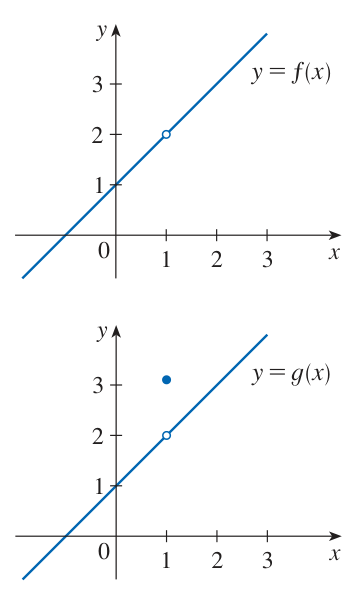
\includegraphics[width=\linewidth]{images/p0133_fig1.png}
    
    \vspace{4pt}
    \begin{flushleft}
    \small
    \textbf{\textsf{HÌNH 2}}\\[2pt]
    Đồ thị của các hàm số $f$ (từ Ví dụ~3) và $g$ (từ Ví dụ~4)
    \end{flushleft}
\end{minipage}%
\hfill
% ==========================================
% CỘT CHÍNH: Nội dung bài học, Ví dụ, Công thức
% ==========================================
\begin{minipage}[t]{0.71\textwidth}
    \vspace*{0pt}
    Các hàm số có Tính chất Thay thế Trực tiếp được gọi là \textit{liên tục tại $a$} và sẽ được nghiên cứu trong Mục~2.5. Tuy nhiên, không phải mọi giới hạn đều có thể tính được ngay từ đầu bằng phương pháp thay thế trực tiếp, như các ví dụ sau đây sẽ chỉ ra.

    \vspace{0.25cm}
    \noindent
    \textbf{\textsf{\color{stewartcyan}VÍ DỤ 3}} \quad Tìm $\displaystyle \lim_{x \to 1} \frac{x^2 - 1}{x - 1}$.

    \vspace{0.15cm}
    \noindent
    \textbf{\textsf{\color{stewartcyan}LỜI GIẢI}} \quad Đặt $f(x) = (x^2 - 1)/(x - 1)$. Ta không thể tìm giới hạn bằng cách thay trực tiếp $x = 1$ vì $f(1)$ không xác định. Chúng ta cũng không thể áp dụng Quy tắc Thương, bởi vì giới hạn của mẫu số bằng~0. Thay vào đó, chúng ta cần thực hiện một số biến đổi đại số sơ bộ. Ta phân tích tử số thành hiệu hai bình phương:
    \[
    \frac{x^2 - 1}{x - 1} = \frac{(x - 1)(x + 1)}{x - 1}
    \]
    Tử số và mẫu số có chung một nhân tử là $x - 1$. Khi lấy giới hạn khi $x$ tiến dần đến 1, ta luôn có $x \neq 1$ và do đó $x - 1 \neq 0$. Vì vậy, ta có thể triệt tiêu nhân tử chung $x - 1$, rồi sau đó tính giới hạn bằng cách thay thế trực tiếp như sau:
    \begin{align*}
    \lim_{x \to 1} \frac{x^2 - 1}{x - 1} &= \lim_{x \to 1} \frac{(x - 1)(x + 1)}{x - 1} \\[5pt]
    &= \lim_{x \to 1} (x + 1) = 1 + 1 = 2
    \end{align*}
    Giới hạn trong ví dụ này đã từng xuất hiện trong Ví dụ~2.1.1 khi tìm tiếp tuyến của parabol $y = x^2$ tại điểm $(1, 1)$. \hfill {\color{stewartcyan}\rule{1.1ex}{1.1ex}}

    \vspace{0.25cm}
    \noindent
    \textbf{\textsf{\color{stewartcyan}GHI CHÚ}} \quad Trong Ví dụ~3, chúng ta đã có thể tính được giới hạn bằng cách thay thế hàm số đã cho $f(x) = (x^2 - 1)/(x - 1)$ bằng một hàm số đơn giản hơn là $g(x) = x + 1$, có cùng giá trị giới hạn. Điều này hoàn toàn hợp lệ vì $f(x) = g(x)$ ngoại trừ khi $x = 1$, mà khi tính giới hạn khi $x$ tiến dần đến 1, chúng ta không quan tâm điều gì xảy ra khi $x$ thực sự \textit{bằng}~1. Nói một cách tổng quát, ta có tính chất hữu ích sau đây.

    \vspace{0.2cm}
    \begin{tcolorbox}[
        colback=white,
        colframe=stewartred,
        arc=0mm,
        boxrule=0.8pt,
        left=10pt,
        right=10pt,
        top=7pt,
        bottom=7pt
    ]
    Nếu $f(x) = g(x)$ khi $x \neq a$, thì $\displaystyle \lim_{x \to a} f(x) = \lim_{x \to a} g(x)$, với điều kiện các giới hạn này tồn tại.
    \end{tcolorbox}

    \vspace{0.2cm}
    \noindent
    \textbf{\textsf{\color{stewartcyan}VÍ DỤ 4}} \quad Tìm $\displaystyle \lim_{x \to 1} g(x)$, trong đó
    \[
    g(x) = \begin{cases}
    x + 1 & \text{nếu } x \neq 1 \\[3pt]
    \pi & \text{nếu } x = 1
    \end{cases}
    \]

    \vspace{0.15cm}
    \noindent
    \textbf{\textsf{\color{stewartcyan}LỜI GIẢI}} \quad Ở đây hàm số $g$ được xác định tại $x = 1$ và $g(1) = \pi$, nhưng giá trị của một giới hạn khi $x$ \textit{tiến đến} 1 không phụ thuộc vào giá trị của hàm số \textit{tại} 1. Vì $g(x) = x + 1$ với $x \neq 1$, ta có
    \[
    \lim_{x \to 1} g(x) = \lim_{x \to 1} (x + 1) = 2 \tag*{\color{stewartcyan}\rule{1.1ex}{1.1ex}}
    \]

    \vspace{0.15cm}
    \noindent
    Lưu ý rằng giá trị của các hàm số trong Ví dụ~3 và 4 là giống hệt nhau ngoại trừ tại điểm $x = 1$ (xem Hình~2), do đó chúng có cùng một giới hạn khi $x$ tiến dần đến~1.
\end{minipage}

\vfill
\begin{center}
\fontsize{6.5pt}{8pt}\selectfont\color{stewartgray}
Copyright 2021 Cengage Learning. All Rights Reserved. May not be copied, scanned, or duplicated, in whole or in part. WCN 02-200-203\\[1pt]
Due to electronic rights, some third party content may be suppressed from the eBook and/or eChapter(s). Editorial review has deemed that any suppressed content does not materially affect the overall learning experience. Cengage Learning reserves the right to remove additional content at any time if subsequent rights restrictions require it.
\end{center}
